\chapter{Visionen und Ziele}
\label{cha:visi}

\paragraph{/V10/} Das Multicast Test Tool soll dazu beitragen die Hardware und
die Software eines Local-Area-Netzwerkes zu verifizieren um die Synchronit"at
und den Gleichlauf des Netzwerkes zu verbessern.

\paragraph{/V20/} Die Multicasting-Fähigkeiten einer Netzwerkinfrastruktur auf
einen Blick erfass- und validierbar machen.

\paragraph{/Z10/} Das Programm soll es den Benutzer erm"oglichen simultan
mindestens 30 Multicasts in einem Local-Area-Netzwerkes zu versenden und zu
empfangen und dabei die Geschwindigkeit, Empfangsintervalle sowie verlorene Pakete zu ermitteln.

\paragraph{/Z20/} Das Tool soll plattformunabhängig sein, um den Blick auf das
Netzwerk von verschiedenen Knoten aus zu ermöglichen.

\paragraph{/Z30/} Eine übersichtliche Oberfläche die sowohl Sender- als auch
Empfängerprogramm zusammenfasst soll eine schnelle Einarbeitung und klare
Bedienung ermöglichen.

%owner jeff

\chapter{Rahmenbedingungen}
\label{cha:rahm}

\section{Organisatorische Rahmenbedingungen}
\label{sec:orga}

\paragraph{Anwendungsbereich:} Netzwerkaufbau, -analyse, -verifikation

\paragraph{Zielgruppen:} Systemtester, Analysten von Netzwerk Hardware bzw.
Netzwerk Software. Die Software wird eingesetzt um die
Multicasting-Fähigkeit des Netzwerks zu analysieren und Aussagen über
Gleichlauf und Zuverlässigkeit machen zu können.

\paragraph{Betriebsbedingungen:} Computer-Netzwerke jeder Ausprägung auf
IP-Basis

\section{Technische Rahmenbedingungen}
\label{sec:tech}

\paragraph{Software:} Die Software unterstützt Windows (ab XP) und Linux. 
Verwendung unter anderen Betriebssystemen mit kompatiblem Java
Runtime Environment und IP-Stack ist prinzipiell möglich, wird aber nicht
garantiert. Ein Java Runtime Environment der Version 6 muss verfügbar sein. Für
die Nutzung der graphischen Nutzeroberfläche ist ebenfalls eines der
Standardfenstersysteme der unterstützen Betriebssysteme notwendig (Windows
Fenstersystem, X.org, Qwartz).

\paragraph{Hardware:} Minimale Anforderung ist ein handels"ublicher Desktop
Computer bzw. Notebook mit Netzwerkkarte(mind. 100mbit/s). Der Computer muss
lokal oder per Netzwerk steuerbar sein.

\paragraph{Orgware:} Ein Anwender kann sowohl Client als auch Server zur selben Zeit darstellen. Eine Netzwerkverbindung zum selben LAN vom Sender auch als Empf"anger ist f"ur das Testen erforderlich.

\section{Anforderungen an die Entwicklungsumgebung}
\label{sec:anf}

\paragraph{Software} Zur Entwicklung eignet sich jedes aktuelle Betriebssystem
mit verfügbarem Java Development Kit der Version 6. Als Entwicklungsumgebung
muss Eclipse in aktueller Version verfügbar sein. In Betriebssystem sowie
Entwicklungsumgebung sollte das verteilte Versionierungssystem Mercurial zum
Verwalten von Systemkomponenten und -dokumenten verfügbar sein. Zugang zum
Internet, sowie ein aktueller Webbrowser sind notwendig, um auf Versionierung
und Projektverwaltung zuzugreifen. Die UML-Software VisualParadigm ist notwendig zur graphischen
Modellierung des Systems.

\paragraph{Hardware} Anforderungen an die Hardware sind identisch zu den
oben genannten.

\paragraph{Orgware} Aufgaben werden online in dem Projekt-Organisations-Werkzeug
Redmine verwaltet. Zugang zu diesem ist für produktive Entwicklung notwendig.
Die graphische Modellierung des Systems erfolgt in UML. Alle Dokumente und
Softwareteile des Systems werden mit dem verteilen Versionierungssystem
Mercurial verwaltet.


% owner: jeff
\chapter{Kontext und "Uberblick}
\label{cha:kont}

\paragraph{Systemumgebung}
Das System wird in einem bereits bestehenden Computer-Netzwerk verwendet. Zu
diesem gehören sowohl die einzelnen Computer als Netzwerkknoten, als auch
sämtliche Peripherie zum Verbinden dieser Knoten untereinander. Das System
ist auf Empfangsseite mit älteren Versionen
der MultiCast-Testing-Software kompatibel.

\paragraph{Systemgrenze}
Das System ist klar auf die Anwendungsschicht beschränkt. Es sollen weder auf
Hardware- noch Betriebssystemebene neue Multicasting-Fähigkeiten implementiert, sondern ausschließlich bereits vorhande Implementierungen genutzt und
getestet werden. Interaktion mit anderen Softwarekomponenten auf
Schnittstellenebene ist nich vorgesehen.

\paragraph{Kontext}
\begin{figure}

\includegraphics[width=10cm]{images/kontext-usecase.png}
\centering
\caption{Grundsätzlicher Anwendungsfall}
\end{figure}
Das System wird auschließlich in lokalen Netzwerken (LAN) verwendet - eine
Verwendung über Internetverbindungen hinweg ist nicht vorgesehen.
Empfangsintervall- und Traversierungszeiten sind in Auflösung von Millisekunden
zu ermitteln. Da Multicast fest im IP-Protokoll spezifiziert ist, wird davon
ausgegangen, dass alle am Netzwerk beteiligten Komponenten dessen Methoden
vollständig unterstützen. Dazu gehört auch auch das
Multicast-Gruppenverwaltungsprotokoll IGMP. Auch bei diesem wird davon
ausgegangen, dass alle beteiligten Netzwerkkomponenten es unterstützen. Sollte
dies nicht der Fall sein, wird kein Mutlicastverkehr stattfinden.


\chapter{Funktionale Anforderungen}
\label{cha:funct}
%TODO Gui-USE Cases einbinden

\section{Übersicht der Anwendungsfälle}
\label{sec:usec}

\begin{figure}[H]
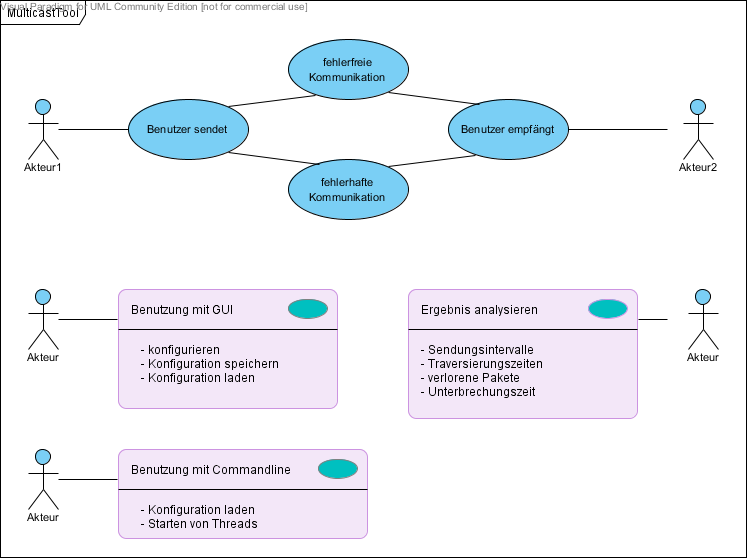
\includegraphics[width=15cm]{images/UseCasesUML.png}
\label{img:usecasesuml}
\caption{Anwendungsfälle}
\end{figure}

\clearpage

\paragraph{/UC10/} Benutzung mit GUI\newline
\texttt{Ziel:} Benutzung des Multicast Test Tools mit grafischem
Userinterface\newline \texttt{Akteure:} Akteur\newline
\texttt{Auslösendes Ereignis:} Akteur startet Programm\newline
\texttt{Beschreibung:}
\begin{itemize}
 \item[-] Starten des Multicast Test Tools mit GUI
 \item[-] Konfiguration des Multicast Test Tools
 \item[-] Speichern einer Konfiguration in Datei
 \item[-] Laden einer Konfiguration aus Datei
\end{itemize}
\texttt{Alternativen:}
\begin{itemize}
 \item[-] Starten des Multicast Test Tools via Commandline
\end{itemize}
\texttt{Testbarkeit:} Starten des Programms


\paragraph{/UC20/} Benutzung via Commandline\newline
\texttt{Ziel:} Benutzung des Multicast Test Tools via Commandline\newline
\texttt{Akteure:} Akteur\newline
\texttt{Auslösendes Ereignis:} Akteur startet Programm\newline
\texttt{Beschreibung:}
\begin{itemize}
 \item[-] Starten des Multicast Test Tools via Commandline
 \item[-] Laden einer Konfiguration von Datei
 \item[-] Starten von Threads
\end{itemize}
\texttt{Alternativen:}
\begin{itemize}
 \item[-] Starten des Multicast Test Tools mit GUI
\end{itemize}
\texttt{Testbarkeit:} Starten des Programms


\paragraph{/UC30/} Benutzer sendet/Benutzer empfängt\newline
\texttt{Ziel:} Testen der Kommunikationsfähigkeit des Netzwerks
\texttt{Akteure:} Akteur1, Akteur2\newline
\texttt{Auslösendes Ereignis:} Starten des Sende- und des
Empfangsvorgangs\newline 
\texttt{Beschreibung:}
\begin{itemize}
 \item[-] Akteur1 sendet Pakete\
 \item[-] Akteur2 versucht Pakete zu empfangen
 \item[-]Kommunikation funktioniert fehlerfrei
\end{itemize}
\texttt{Alternativen:}
\begin{itemize}
  \item[-] Kommunikation ist fehlerhaft, d.h. einige oder alle Pakete gehen
  verloren
\end{itemize}
\texttt{Testbarkeit:} Senden von Paketen zur Überprüfung und Analysieren der
Ergebnisse


\paragraph{/UC40/} Ergebnis analysieren\newline
\texttt{Ziel:} Untersuchung des Netzwerkverhaltens\newline
\texttt{Akteure:} Akteur\newline
\texttt{Auslösendes Ereignis:} Anzeige der Ergebnisse durch das
Multicast Test Tool\newline
\texttt{Beschreibung:}
\begin{itemize}
  \item[-] Analyse der Sendungsintervalle
  \item[-] Analyse der Traversierungszeiten
  \item[-] Analyse der Anzahl der verlorenen Pakete
  \item[-] Analyse der Unterbrechungszeit
\end{itemize}
\texttt{Alternativen:} -\newline
\texttt{Testbarkeit:} Test noch mal durchführen\newline

\clearpage

\section{Verpflichtende Anforderungen}
\label{sec:mandatory}

%TODO Beschreibung konkretisieren

\subsection{Statik}
\label{sec:statik}

\paragraph{/VA0100/ (/LVA0100/)} Multicast-Sendefähigkeit\\
\texttt{Beschreibung:} Das System muss neue IP-Multicast-Gruppen öffnen und
Testströme von UDP-Paketen beliebiger Größe (bis zur Jumbo-Paket-Grenze von
9000bytes) auf beliebigen Ports in Millisekunden-Intervallen versenden können.\\
\texttt{Anforderungsschicht:} Statik/Dynamik\\
\texttt{Priorität:} sehr hoch\\
\texttt{Stabilität:} fest\\
\texttt{Aufwand:} 2 Personentage\\
\texttt{Entwicklungsrisiko:} hoch\\
\texttt{Version und "Anderungsbeschreibung:}

\paragraph{/VA0200/ (/LVA0200/)} Multicast-Empfangsfähigkeit\\
\texttt{Beschreibung:} Das System muss bestehende Multicast-Gruppen
per IGMP abonnieren und Testströme von UDP-Paketen auf beliebigen Ports in
Millisekunden-Intervallen empfangen und deren Eingang protokollieren können.\\
\texttt{Anforderungsschicht:} Statik/Dynamik\\
\texttt{Priorität:} sehr hoch\\
\texttt{Stabilität:} fest\\
\texttt{Aufwand:} 2 Personentage\\
\texttt{Entwicklungsrisiko:} hoch\\
\texttt{Version und "Anderungsbeschreibung:}

\paragraph{/VA0300/ (/LVA0400/)} Gleichzeitigkeit\\
\texttt{Beschreibung:} Das System muss auf einem handelsüblichen Rechner
mindestens 30 Datenströme gleichzeitig senden und empfangen können.\\
\texttt{Anforderungsschicht:}Statik/Dynamik\\
\texttt{Priorität:} hoch\\
\texttt{Stabilität:} fest\\
\texttt{Aufwand:} 2 Personentage\\
\texttt{Entwicklungsrisiko:} hoch\\
\texttt{Version und "Anderungsbeschreibung:}

\paragraph{/VA0400/ (/LVA0500/)} Kompatibilität\\
\texttt{Beschreibung:} Das System muss auf Empfangsseite
mit den Datenströmen des Multicast Test Tools der Hirschmann Automation GmbH
kompatibel sein.\\
\texttt{Anforderungsschicht:} Statik\\
\texttt{Priorität:} hoch\\
\texttt{Stabilität:} gefestigt\\
\texttt{Aufwand:} 3 Personentage\\
\texttt{Entwicklungsrisiko:} mittel\\
\texttt{Version und "Anderungsbeschreibung:}

\paragraph{/VA0500/ (/LVA0600/)} Konfigurierbarkeit\\
\texttt{Beschreibung:} Die Sendekomponente des System muss in folgenden
Punkten konfigurierbar sein: Paketgröße (einschließlich Jumbo-Pakete),
Paket-Senderate, Time-to-live (TTL), Multicast-Gruppe, Port, Nutzdaten
(Zeichenkette), Paketformat\\
\texttt{Anforderungsschicht:} Statik\\
\texttt{Priorität:} hoch\\
\texttt{Stabilität:} gefestigt\\
\texttt{Aufwand:} 2 Personentage\\
\texttt{Entwicklungsrisiko:} hoch\\
\texttt{Version und "Anderungsbeschreibung:}

\paragraph{/VA0600/ (/LVA0800/)} Konfigurationsdatei\\
\texttt{Beschreibung:} Das System muss die Einstellungen zu allen gebotenen
Funktionalitäten in einer Konfigurationsdatei persistieren und aus dieser
wiederherstellen können. Die Konfigurationsdatei soll im XML-Format vorliegen
und syntaktisch leicht verständlich sein, damit der Benutzer sie auch per Hand
erstellen oder ändern kann.\\
\texttt{Anforderungsschicht:} Statik\\
\texttt{Priorität:} hoch\\
\texttt{Stabilität:} gefestigt\\
\texttt{Aufwand:} 3 Personentage\\
\texttt{Entwicklungsrisiko:} mittel\\
\texttt{Version und "Anderungsbeschreibung:}

\paragraph{/VA0700/ (/LVA0900/)} Grafische Nutzeroberfläche\\
\texttt{Beschreibung:} Das System muss sowohl unter Linux, als auch unter
Windows eine einheitliche Benutzeroberfläche bieten, die den Zugriff auf alle Funktionen
des Programms ermöglicht.\\
\texttt{Anforderungsschicht:} Statik\\
\texttt{Priorität:} mittel\\
\texttt{Stabilität:} fest\\
\texttt{Aufwand:} 14 Personentage\\
\texttt{Entwicklungsrisiko:} mittel\\
\texttt{Version und "Anderungsbeschreibung:}

\paragraph{/VA0800/ (/LVA1000/)} Zusammenfassung von Sende- und
Empfangsfunktionalität\\
\texttt{Beschreibung:} Das System muss Sende- und Empfangsfunktionalität
unter derart vereinigen, dass beide Funktionalitäten gemeinsam verteilbar und
steuerbar sind.\\
\texttt{Anforderungsschicht:}
Statik\\ \texttt{Priorität:} mittel\\
\texttt{Stabilität:} fest\\
\texttt{Aufwand:}\\
\texttt{Entwicklungsrisiko:} mittel\\
\texttt{Version und "Anderungsbeschreibung:}

\paragraph{/VA0900/ (/LVA1300/)} Textbasierte Nutzeroberfläche\\
\texttt{Beschreibung:} Das System muss dem Anwender mit einer konsolenbasierten
Nutzerschnittstelle die Steuerung aller Programmfunktionen per
Konfigurationsdatei oder Parametern ermöglichen. Die Konsolenschnittstelle muss
intuitiv in Skripten eingebunden werden können. Die Ergebnisse müssen in einfach weiterzuverarbeiten
Logdateien festgehalten werden.\\
\texttt{Anforderungsschicht:} Statik\\
\texttt{Priorität:} mittel\\
\texttt{Stabilität:} fest\\
\texttt{Aufwand:} 14 Personentage\\
\texttt{Entwicklungsrisiko:} mittel\\
\texttt{Version und "Anderungsbeschreibung:}

\subsection{Dynamik}
\label{sec:dynamik}

\paragraph{/VA1000/ (/LVA0700/)} Sendestatistik\\
\texttt{Beschreibung:} Die Sendekomponente des System muss laufende
Informationen zu folgenden Punkten ausgeben: Anzahl der gesendeten Pakete
(gesamt, pro MC-Gruppe), Paketraten (gesamt, pro MC-Gruppe), per Zufall
generierte Sender-Identifikationsnummer\\
\texttt{Anforderungsschicht:} Dynamik\\
\texttt{Priorität:} hoch\\
\texttt{Stabilität:} gefestigt\\
\texttt{Aufwand:} 1 Personentage\\
\texttt{Entwicklungsrisiko:} mittel\\
\texttt{Version und "Anderungsbeschreibung:}

\paragraph{/VA1100/ (/LVA1100/)} Darstellung der Sendeströme\\
\texttt{Beschreibung:} Ausgehende Multicast-Datenströme müssen mit ihren
Parametern in einer Liste angezeigt werden. Die Ströme müssen in der Liste
direkt per Mausklick aktivierbar und deaktivierbar sein. Die Liste soll es dem
Anwender außerdem erlauben, die Parameter mehrerer Sendeströme gleichzeitig zu
bearbeiten.\\
\texttt{Anforderungsschicht:} Dynamik/Statik\\
\texttt{Priorität:} mittel\\
\texttt{Stabilität:} volatil\\
\texttt{Aufwand:}\\
\texttt{Entwicklungsrisiko:} mittel\\
\texttt{Version und "Anderungsbeschreibung:}

\paragraph{/VA1200/ (/LVA1200/)} Messwertanzeige\\
\texttt{Beschreibung:} Die grafische Oberfläche muss die nach /VA1300/
ermittelten Messwerte als dem jeweiligen Datenstrom eindeutig zugehörig
darstellen.\\
\texttt{Anforderungsschicht:} Dynamik/Statik\\
\texttt{Priorität:} mittel\\
\texttt{Stabilität:} fest\\
\texttt{Aufwand:} 3 Personentage\\
\texttt{Entwicklungsrisiko:} mittel\\
\texttt{Version und "Anderungsbeschreibung:}

\subsection{Logik}
\label{sec:logik}

\paragraph{/VA1300/ (/LVA0300/)} Datenauswertung\\
\texttt{Beschreibung:} Die Empfangskomponente des Systems muss Daten bezüglich
folgender Punkte bereitstellen: Anzahl und Dauer von Unterbrechungen, Paketrate
(gesamt, pro MC-Gruppe), Anzahl empfangener Pakete (gesamt, pro MC-Gruppe),
Anzahl verlorener Pakete (gesamt, pro MC-Gruppe), Empfang fehlerhafter Pakete\\
\texttt{Anforderungsschicht:} Logik\\
\texttt{Priorität:} hoch\\
\texttt{Stabilität:} gefestigt\\
\texttt{Aufwand:} 3 Personentage\\
\texttt{Entwicklungsrisiko:} hoch\\
\texttt{Version und "Anderungsbeschreibung:}

\section{Optionale Anforderungen}
\label{sec:optional}


\paragraph{/OA0100/ (/LOA0100/)} IPV6 Unterstützung\\
\texttt{Beschreibung:} Das Programm soll in Zukunft fähig sein Multicasts in
IPV6 Netzwerken testen zu können.\\
\texttt{Anforderungsschicht:} Statik\\ 
%Querbez"uge: keine \\
\texttt{Abnahmekriterien:} Das Programm in einer IPV6 Umgebung testen.\\
\texttt{Priorit"at:} Niedrig\\
\texttt{Stabilit"at:} Fest\\
\texttt{Aufwand:} 5 Personentage\\
\texttt{Entwicklungsrisiko:} Mittel\\
\texttt{Version und "Anderungsbeschreibung:}\newline

\paragraph{/OA0200/ (/LOA0200/)} NTP Zeitsynchronisierung\\
\texttt{Beschreibung:} Verschiedene Sender und Empfänger sollen in Zukunft
ihre Zeit über NTP synchronisieren um die Traversierungszeit von Paketen
ermitteln zu können.\\ 
\texttt{Anforderungsschicht:} Statik\\ 
\texttt{Abnahmekriterien:} Die Zeitsynchronisierung in den Logdateien
nachvollziehen.\\ 
\texttt{Priorit"at:} Niedrig\\
\texttt{Stabilit"at:} Volatil\\
\texttt{Aufwand:} 2 Personentage\\
\texttt{Entwicklungsrisiko:} Mittel\\
\texttt{Version und "Anderungsbeschreibung:}

\paragraph{/OA0300/ (/LOA0300/)} Darstellung der Messergebnisse\\
\texttt{Beschreibung:} Die Messergebnisse sollen mithilfe von Farbcodes oder
Grafiken präsentiert werden. Verlorene Pakete und Geschwindigkeitsunterschiede
sollen so auf einen Blick erfassbar gemacht werden.\\
\texttt{Anforderungsschicht:} Statik\\ 
\texttt{Abnahmekriterien:} Durchführen von Messungen und validieren der
generierten Grafiken anhand der ausgegebenen Messwerte.\\ 
\texttt{Priorit"at:} Niedrig\\
\texttt{Stabilit"at:} Volatil\\
\texttt{Aufwand:} 2 Personentage\\
\texttt{Entwicklungsrisiko:} Mittel\\
\texttt{Version und "Anderungsbeschreibung:}

\paragraph{/OA0400/ (/LOA0400/)} Nutzdatenübertragung\\
\texttt{Beschreibung:} In Zukunft soll es möglich sein Nutzdaten in den
UDP-Datagrammen zu übertragen.\\
\texttt{Anforderungsschicht:} Statik\\ 
\texttt{Abnahmekriterien:} Übertragung von Nutzdaten und validieren der Daten
nach der Übertragung mit Hilfe eines Hash-Wertes.\\
\texttt{Priorit"at:} Niedrig\\
\texttt{Stabilit"at:} Volatil\\
\texttt{Aufwand:} 1 Personentag\\
\texttt{Entwicklungsrisiko:} Gering\\
\texttt{Version und "Anderungsbeschreibung:}

\chapter{Qualit"atsanforderungen}
\label{cha:qual}

\begin{table}[htdp]
\caption{Definition der Qualit"atsanforderungen}
\label{tab:quality}
\begin{center}
\begin{tabular}{|l|c|c|c|c|}
\hline
\textbf{Systemqualit"at} & \textbf{sehr gut} & \textbf{gut} & \textbf{normal} & \textbf{nicht relevant} \\
\hline
Funktionalit"at & & x & & \\
\hline
Zuverl"assigkeit & & x & & \\
\hline
Benutzbarkeit & & x & & \\
\hline
Effizienz & & x & & \\
\hline
Wartbarkeit & & & x & \\
\hline
Portabilit"at & x & & &  \\
\hline
\end{tabular}
\end{center}
\label{default}
\end{table}

\section{Funktionalit"at}

\paragraph{/LQF10/} Die Funktionalität des Systems soll in einer einzelnen
Programmdatei zusammengefasst werden.

\paragraph{/LQF20/} Die vollständige Funktionalität des
Multicast Test Tool der Hirschmann Automation GmbH soll auch im neuen
Produkt verfügbar sein.

\paragraph{/LQF30/} Die vollständige Funktionalität des Systems muss auch über
die Kommandozeile erreichbar sein.

\paragraph{/LQF40/} Das Produkt soll empfangsseitig kompatibel zum
Multicast Test Tool der Hirschmann Automation GmbH sein. Siehe hierzu auch /VA0500/
 
\section{Zuverl"assigkeit}

\paragraph{/LQZ10/} Die Software darf bei fehlerhafter Konfiguration durch den
Benutzer nicht abstürzen.

\paragraph{/LQZ20/} Die Software darf nicht durch fehlerhafte Implementation von
Multicasting-Protokollen in den Netzwerkkomponenten zum Absturz gebracht werden.

\paragraph{/LQZ30/} Alle gesendeten Datenpakete müssen unter allen Umständen dem
Protokoll der Anwendung gehorchen. Analog müssen alle unbeschädigt empfangenen
Datenpakete korrekt nach dem Protokoll der Anwendung weiterverarbeitet werden.

\paragraph{/LQZ40/} Beschädigte Pakete, oder solche, die dem Anwendungsprotokoll
nicht gehorchen, sollen trotzdem, soweit es die enthaltenen Daten noch zulassen,
weiterverarbeitet und ausgewertet werden.

\paragraph{/LQZ50/} Innerhalb der Messdatenverarbeitung dürfen keine
Rundungs- und Berechnungsfehler auftreten, die eine Messgenauigkeit von 5
Millisekunden beeinträchtigen.

\section{Benutzbarkeit}

\paragraph{/LQU10/} Die grafische Oberfläche soll sich an das Multicast Test
Tool der Hirschmann Automation GmbH anlehnen.

\paragraph{/LQU20/} Die Multicasting-Ströme sollen übersichtlich in einer Liste
angezeigt werden.

\paragraph{/LQU30/} Ein Multicasting-Strom soll mit einem Mausklick direkt in
der Liste aus /LQU20/ aktiviert und deaktiviert werden können.

\paragraph{/LQU40/} Die grafische Oberfläche soll gesendete
und empfangene Multicast-Strömen eindeutig optisch trennen.

\paragraph{/LQU50/} Die Parameter der Datenströme sollen intuitiv direkt
bearbeitbar sein. Dies soll auch für mehrere Datenströme gleichzeitig möglich
sein.

\paragraph{/LQU60/} Messergebnisse und ihr Zweck müssen eindeutig präsentiert
werden.

\paragraph{/LQU70/} Das Produkt soll von einem Anwender, der mit dem
Netzwerkhintergrund vertraut ist, schnell erlernbar sein.

\section{Effizienz}

\paragraph{/LQE10/} Auf einem gewöhnlichen Arbeitsrechner (CPU-Takt > 1GHz,
RAM-Kapazität > 1GB, 100Mbit-Netzwerkadapter) müssen mindestens 30
Multicast-Ströme zeitgleich gesendet und empfangen werden können.

\section{Wartbarkeit}

\paragraph{/LQW10/} Die Software soll klar modularisiert sein. Modulgrenzen
müssen eindeutig definiert und die Module selbst austauschbar sein.

\paragraph{/LQW20/} Die Module müssen einzeln testbar, sowie Fehlerzustände
analysierbar sein.

\paragraph{/LQW30/} Schnittstellen zwischen Modulen sind als Interfaces zu
definieren und nach Javadoc-Konventionen zu dokumentieren.

\paragraph{/LQW40/} Schnittstellen für spätere Erweiterungen sollen im Produkt
vorhanden sein.

\section{Portabilität}

\paragraph{/LQP10/} Die Software muss sowohl unter Linux, als auch unter Windows
(ab Windows XP) funktionieren.

\paragraph{/LQP20/} Die Software soll das Netzwerk von verschiedenen Knoten aus
analysierbar machen, darum muss sie auch auf unterschiedlicher Hardware ihre
volle Funktionalität bereitstellen.

\paragraph{/LQP30/} Das Programm soll von einem erfahrenen Benutzer ohne
besondere Vorbereitungen installierbar sein.

\paragraph{/LQP40/} Die Software darf, wenn sie gemeinsam mit anderen Programmen
auf demselben Gerät betrieben wird, keine Konflikte erzeugen. Dies gilt
insbesondere dann, wenn die Fremdsoftware ähnliche Aufgaben, wie das Produkt
erfüllt.